%! Author = Nandakishore Vinayakrishnan
%! Date = 22/11/2026
% =====================================================================
%  MSc Dissertation Interim Report
%  Formatted with the IEEE conference template (IEEEtran.cls) and the
%  IEEEtran BibTeX style, both loaded from the template folders at the
%  repository root:
%    ../conference-latex-template/IEEE-conference-template-062824/IEEEtran.cls
%    ../IEEEtranBST2/IEEEtran.bst
%
%  Build (from src/):  latexmk -pdf main.tex   (settings in src/latexmkrc)
%     or:  pdflatex main -> bibtex main -> pdflatex main -> pdflatex main
% =====================================================================
\documentclass[conference,a4paper]{../conference-latex-template/IEEE-conference-template-062824/IEEEtran}
\IEEEoverridecommandlockouts

% ---------- Packages (as in the IEEE template, plus those this report needs) ----------
\usepackage{cite}
\usepackage{amsmath,amssymb,amsfonts}
\usepackage{graphicx}
\usepackage{textcomp}
\usepackage{xcolor}
\usepackage{booktabs}
\usepackage{tabularx}
\usepackage{array}
\usepackage{enumitem}
\usepackage{float}
\usepackage{listings}
\usepackage{tikz}
\usetikzlibrary{positioning,arrows.meta,fit,backgrounds,shapes.geometric}
\usepackage{pgfgantt}
\usepackage[hidelinks]{hyperref}

% ---------- Styling ----------
\definecolor{accent}{HTML}{1F4E79}
\definecolor{todo}{HTML}{C00000}
\definecolor{codebg}{HTML}{F5F7FA}
\newcolumntype{Y}{>{\raggedright\arraybackslash}X}
\setlist{itemsep=1pt, topsep=3pt}

\lstset{
    basicstyle=\ttfamily\scriptsize,
    backgroundcolor=\color{codebg},
    frame=single, rulecolor=\color{black!15},
    breaklines=true, columns=fullflexible,
    keywordstyle=\color{accent}\bfseries,
    commentstyle=\color{black!55}\itshape,
    showstringspaces=false
}

% ---------- Draft markers ----------
\newif\ifdraft
\drafttrue
\newcommand{\todoin}[1]{\ifdraft{\color{todo}\footnotesize[\textbf{TODO:} #1]}\fi}

% ---------- Administrative details (edit here) ----------
\newcommand{\reporttitle}{Role-Adaptive Digital Shadow Dashboard for Real-Time Battery Management System Verification}
\newcommand{\studentname}{Nandakishore Vinayakrishnan}
\newcommand{\studentid}{23070854}
\newcommand{\programme}{MSc Immersive Software Engineering}
\newcommand{\supervisorname}{Marie Travers}
\newcommand{\supervisoremail}{marie.travers@ul.ie}
\newcommand{\industrypartner}{Analog Devices, BMS System Test Team (STT)}
\newcommand{\artefactrepo}{\url{https://github.com/Nanda128/[artefact-repo]}}
\newcommand{\reportrepo}{\url{https://github.com/Nanda128/Interim-Dissertation}}
\newcommand{\wordcount}{[word count]}
\newcommand{\submissiondate}{December 2026}

\hypersetup{pdftitle={Interim Report: \reporttitle}, pdfauthor={\studentname}}

\begin{document}

    % =====================================================================
% 1. Title Page and Administrative Details
% =====================================================================
\begin{titlepage}
    \centering
    {\small\scshape University of Limerick\\Department of Computer Science and Information Systems\par}
    \vspace{2.5cm}
    {\Large\scshape MSc Dissertation Interim Report\par}
    \vspace{1cm}
    {\LARGE\bfseries\color{accent}\reporttitle\par}
    \vspace{2cm}

    \begin{tabularx}{0.85\textwidth}{@{}lY@{}}
        \toprule
        Student             & \studentname                                                                             \\
        Student number      & \studentid                                                                               \\
        Programme           & \programme                                                                               \\
        Supervisor          & \supervisorname\ (\href{mailto:\supervisoremail}{\texttt{\supervisoremail}})             \\
        Industry partner    & \industrypartner                                                                         \\
        Word count          & \wordcount\ (excluding title page, abstract, tables, figures, references and appendices) \\
        Report repository   & \reportrepo                                                                              \\
        Submitted           & \submissiondate                                                                          \\
        \bottomrule
    \end{tabularx}

    \vfill
\end{titlepage}

    \maketitle
    % =====================================================================
% 2. Abstract / Executive Summary (150-250 words)
% =====================================================================
\begin{abstract}
    Battery management systems (BMS) are verified on hardware-in-the-loop (HIL) rigs that generate large volumes of sensor data.
    At Analog Devices, the industry partner, this data is accessed through raw logs and engineering tools, including an existing analysis GUI, none of which is suited to live monitoring or to presenting results to project leads and customers.
    This project proposes a customer-facing dashboard, designed as a digital shadow of the test rig, for stakeholders ranging from test engineers to visiting customers.
    This dashboard seeks to investigate whether Key Performance Indicators (KPIs) can be streamed from the rig in near-real-time, and how you would filter noisy signals without concealing genuine faults.
    In addition, would role-specific views, matched to each audience's technical expertise reduce task time or visual clutter?
    The dashboard's values are also verified against the partner's validated software.
    The work follows a Design Science Research approach and is evaluated without human participants, using recorded and simulated data containing faults introduced at known times.
    At this stage, the requirements analysis, literature review, system architecture and experimental design are complete.
    Implementation will begin with the prototype phase of the partner's plan.
\end{abstract}

\begin{IEEEkeywords}
    battery management systems, digital shadow, hardware-in-the-loop testing, dashboard design, signal conditioning
\end{IEEEkeywords}


    % =====================================================================
% 3. Introduction and Problem Statement
% =====================================================================
\section{Introduction and Problem Statement}
\label{sec:intro}

Battery management systems monitor cell voltages, currents and temperatures, estimate state of charge, balance cells and protect packs from unsafe operating conditions~\cite{plett2015battery}.
Because BMS failures can lead to thermal events in electric vehicles and energy-storage systems, their verification is safety-relevant and is carried out under functional-safety regimes such as ISO~26262~\cite{iso26262}.
Verification is typically performed on hardware-in-the-loop rigs that emulate a battery pack, its loads and its fault conditions while the BMS under test responds in real time.

At the industry partner, the System Test Team (STT) operates such a rig.
Its outputs are currently available only through raw data logs and engineering interfaces, so engineers rely on scripts and offline analysis to interpret results.
This causes two problems identified in the partner's project brief.
First, \textbf{limited visibility}: anomalies during long validation runs may only be found after a test has finished, which lengthens debugging.
Second, \textbf{poor presentation for stakeholders}: there is no interface suitable for showing test status and key performance indicators (KPIs) to project leads or to customers during visits.

Three groups are affected: test engineers, who need detailed, trustworthy real-time data; project leads, who need to see quickly whether a test met its objectives; and customers, who need a clear, credible view of the team's testing rigour.

Building a dashboard is not technically novel in itself.
What is not well understood is how to build one for this setting that is non-intrusive, faithful to noisy signals and appropriate for several audiences at once, and how to show that it is.
Principles for supervisory displays and alarm management are well established for aviation and process control~\cite{sheridan1992telerobotics,isa2016alarm}, but they assume an operator controlling a physical process.
Verification engineering differs: the operator supervises a \emph{test}, judging whether behaviour meets a specification.
Whether those principles transfer to this setting, and how the trade-off between smoothing noise and preserving fault visibility should be handled, has received little attention.
This project addresses that gap with a working artefact used as the vehicle for evaluation.

    % =====================================================================
% 4. Aims, Objectives and Research Questions
% =====================================================================
\section{Aims, Objectives and Research Questions}
\label{sec:aims}

The aim of this project is to design, implement and evaluate a read-only dashboard that provides engineers, project leads and customers with an accurate and timely view of BMS tests, without interfering with the test rig.
The project is classified as hybrid, in that the system is developed as the means of answering four research questions.

\begin{description}[leftmargin=1.2em, labelindent=0pt, font=\normalfont\bfseries]
    \item[RQ1.] Can a read-only streaming pipeline with interchangeable data adapters deliver KPIs in near real time without measurably affecting the test rig?
    \item[RQ2.] Which filtering methods reduce measurement noise while preserving the visibility of genuine fault transients?
    \item[RQ3.] Can a tiered alert scheme with deduplication, hysteresis and shelving reduce the number of alerts without missing critical faults?
    \item[RQ4.] Do role-specific views reduce predicted task time and visual clutter while satisfying accessibility requirements?
\end{description}

The objectives are as follows:
\begin{enumerate}[label=\textbf{O\arabic*}]
    \item to derive a documented set of requirements from the partner's project brief;
    \item to implement simulator, replay and live-rig adapters behind a common interface;
    \item to generate test traces containing spikes, drifts and dropouts at known times;
    \item to implement and compare at least four filtering methods;
    \item to implement the alert engine and the three role-specific views;
    \item to conduct the four experiments described in Section~\ref{sec:evaluation} and to report the results against the criteria in Table~\ref{tab:success}.
\end{enumerate}

\subsection{Changes since the proposal}\label{subsec:changes-since-the-proposal}
RQ3 has been revised to measure the reduction in alerts directly, rather than by comparison with external industrial targets.
The original timeline also followed the partner's rollout schedule; as deployment, training and go-live are not assessed, the revised plan allocates dedicated time to the experiments (Table~\ref{tab:deliverables}).

\begin{table}[H]
    \centering\small
    \caption{Company and research deliverables. Only the research deliverables are assessed.}
    \label{tab:deliverables}
    \begin{tabularx}{\textwidth}{YY}
        \toprule
        \textbf{Company deliverable} & \textbf{Research deliverable} \\
        \midrule
        GUI deployed on the STT environment & Reference architecture and adapters \\
        Training, go-live and sign-off & Experiment scripts, datasets and results \\
        \bottomrule
    \end{tabularx}
\end{table}

    % =====================================================================
% 5. Literature and Technology Review (Progress to Date)
% =====================================================================
\section{Literature and Technology Review}
\label{sec:literature}

\subsection{Supervisory control and situation awareness}\label{subsec:supervisory-control-and-situation-awareness}
Sheridan~\cite{sheridan1992telerobotics} defines supervisory control as the monitoring of an automated process with intermittent human intervention, a description that closely matches an engineer observing a long BMS test.
Of the four stages of automation identified by Parasuraman et al.~\cite{parasuraman2000model}, a read-only dashboard performs only information acquisition and analysis, so that all decisions concerning the test remain with the engineer.
Endsley's model of situation awareness~\cite{endsley1995toward} distinguishes between the perception of events, their comprehension and the projection of future states.
These levels correspond to the needs of the different audiences: an engineer is chiefly concerned with perceiving changes in individual cells, whereas a project lead requires comprehension of whether the test is proceeding as planned.

\subsection{Digital twins and test benches}\label{subsec:digital-twins}
Kritzinger et al.~\cite{kritzinger2018digital} define a digital shadow as a representation that receives data automatically from a physical object but does not transmit data back to it.
The dashboard is deliberately designed as a digital shadow, since a system without a write path to the rig cannot disturb a running test.
Research on battery digital twins has concentrated on state estimation and degradation, and a recent review identifies the rapid creation of dashboard interfaces as an unresolved challenge~\cite{naseri2023batterydt}.
Monitoring dashboards with alerting exist for experimental test beds, but they are described rather than evaluated~\cite{darkside2025grafana}.
No study was identified that evaluates monitoring software for verification rigs against principles of alarm management or situation awareness.
\todoin{Run and report a documented Scopus query to support this claim.}

\subsection{Alarm management}\label{subsec:alarm-management}
Wang et al.~\cite{wang2016alarmoverview} report that chattering alarms, which repeatedly activate and clear within a short period, may account for between 10\% and 60\% of all alarm occurrences in process plants.
Since a threshold alert on a noisy cell voltage would behave similarly, the alert engine merges duplicate alerts, applies hysteresis and allows engineers to shelve alerts that have already been acknowledged.
Alert colours follow the aviation convention of red for warnings and amber for cautions~\cite{faa2010alerting}, with blue reserved for advisories.

\subsection{Signal conditioning}\label{subsec:signal-conditioning}
The partner's brief requires that filtering should not misrepresent ``short spikes or noise''.
Moving-average and exponential filters suppress noise at low computational cost but attenuate and delay abrupt changes.
Median and Hampel filters remove isolated outliers while preserving sharp edges, although they may also remove a genuine single-sample spike.
Kalman filters are widely applied to BMS state estimation~\cite{plett2015battery}, but they depend on a system model and careful tuning.
Research on BMS sensor faults has largely evaluated model-based observers using a constant sensor bias~\cite{yu2021sensorfault}; no comparison of simpler filters on BMS data with seeded spikes, drifts and dropouts was found, and RQ2 addresses this gap.

\subsection{Evaluation of dashboards without users}\label{subsec:dashboard-evaluation}
Few~\cite{few2013dashboard} argues that monitoring dashboards should fit on a single screen and avoid decorative elements, which is in tension with the brief's request for a polished customer display.
The Keystroke-Level Model (KLM) predicts expert task completion time from standard operator times, with an error of approximately 21\%~\cite{card1980keystroke}; this accuracy is sufficient for comparing alternative designs.
The feature-congestion measure proposed by Rosenholtz et al.~\cite{rosenholtz2007clutter} estimates visual clutter from a screenshot.
Automated WCAG~2.2~\cite{w3c2023wcag} checks cover at most half of the success criteria~\cite{vigo2013benchmarking}, and a manual checklist is therefore also employed.

\subsection{Existing tools and technology choices}\label{subsec:tech}
Commercial HIL software, such as that supplied by dSPACE and NI, provides instrument panels intended for the engineers conducting a test and is tied to the vendor's hardware.
Grafana is the most credible alternative, as it supports time-series panels and alerting with minimal development effort.
However, it lacks built-in support for shelving and hysteresis, and it is poorly suited to producing distinct views for different audiences; it is therefore adopted as a comparison baseline rather than as the implementation platform.
Table~\ref{tab:tech} summarises the principal technology decisions.

\begin{table}[H]
    \centering\small
    \caption{Technology decisions.}
    \label{tab:tech}
    \begin{tabularx}{\textwidth}{llY}
        \toprule
        Decision & Choice & Rationale \\
        \midrule
        Transport & WebSocket & Lower latency than polling~\cite{pimentel2012websocket} \\
        Rig ingestion & Read-only DB polling & Requires no change on the partner's side \\
        Storage & TimescaleDB (provisional) & SQL support; a single database for runs and samples \\
        Front end & React, canvas charts & Full control over role-specific views \\
        Downsampling & MinMaxLTTB & Preserves peaks at low computational cost~\cite{vandonckt2023minmaxlttb} \\
        \bottomrule
    \end{tabularx}
\end{table}

The remaining review will cover a documented database search for the research gap, the BMS fault types most relevant to the STT, and benchmarks for time-series databases and chart rendering.

    % =====================================================================
% 6. Requirements and Scope
% =====================================================================
\section{Requirements and Scope}
\label{sec:requirements}

The requirements were derived from the partner's project brief.
Each goal was decomposed into testable requirements linked to a research question, which will be validated with the STT before implementation.
The complete specification of 11 functional and 8 non-functional requirements is provided in Appendix~\ref{sec:trace}.

Three personas were defined.
The \textbf{test engineer} requires visibility of every cell, raw and filtered signals side by side, and early warning of anomalies.
The \textbf{project lead} requires a clear pass or fail outcome supported by the key figures.
The \textbf{customer} encounters the system during a laboratory visit, where it is presented by an engineer.

The essential functional requirements are interchangeable data sources (FR1), KPIs such as pack voltage and cell-voltage spread (FR2), reuse of the STT's calibration code (FR3), near-real-time streaming (FR4), filtering with raw data always retained (FR5), the alert engine (FR6), three role-specific views (FR7) and demonstration replay (FR8).
The principal non-functional requirement is that the dashboard never writes to the rig and imposes negligible load on it (NFR1).
Further targets include an end-to-end latency below 500\,ms (NFR2) and compliance with WCAG~2.2 AA (NFR5).

The project does not modify test procedures or hardware, control the rig, employ machine learning or involve human participants.
Deployment and training constitute company work and fall outside the scope of the dissertation.

    % =====================================================================
% 7. Methodology and Development Approach
% =====================================================================
\section{Methodology and Development Approach}
\label{sec:methodology}

The project adopts Design Science Research~\cite{hevner2004design}, in which an artefact is constructed to address a practical problem and is subsequently subjected to rigorous evaluation.
The evaluation is entirely system-based.
Each experiment uses recorded or simulated data with faults at known times, so results can be checked against ground truth and reproduced.
Success criteria are fixed before any results are obtained.

Most of the data will be produced by a BMS simulator developed for this project, while the NASA battery data set~\cite{saha2007battery} will be replayed to provide realistic background signals.
Partner traces will be used internally only, and reported results will be based on simulated or public data unless the partner agrees otherwise.

Development uses two-week iterations, with live feature tracking, and continuous integration tests and automated accessibility checks.

As no human participants are involved and no personal data are collected, ethics approval is not expected to be required.

    % =====================================================================
% 8. Design and Architecture
% =====================================================================
\section{Design and Architecture}
\label{sec:design}

The system comprises three layers, with data flowing exclusively from the rig towards the browser (Figure~\ref{fig:architecture}).
No component is able to issue commands to the rig, and NFR1 is therefore satisfied by the structure of the system itself.

\begin{figure}[H]
    \centering
    \resizebox{\textwidth}{!}{% High-level architecture: three layers, adapters, one-way data flow.
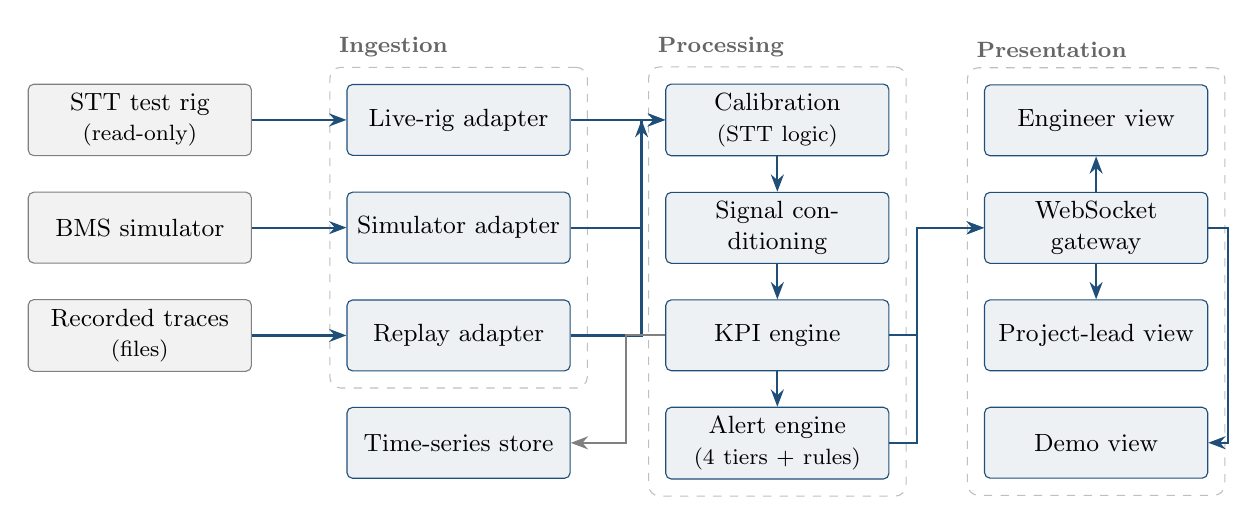
\begin{tikzpicture}[
  font=\small,
  box/.style={draw=accent, fill=accent!8, rounded corners=2pt, align=center, minimum height=0.9cm, text width=2.6cm},
  ext/.style={draw=black!50, fill=black!5, rounded corners=2pt, align=center, minimum height=0.9cm, text width=2.6cm},
  layer/.style={draw=black!25, dashed, rounded corners=4pt, inner sep=6pt},
  lbl/.style={font=\footnotesize\bfseries\color{black!60}, anchor=south west},
  flow/.style={-{Stealth[length=2.2mm]}, thick, accent},
  node distance=0.45cm and 0.6cm
]
% Sources
\node[ext] (rig) {STT test rig\\\footnotesize(read-only)};
\node[ext, below=of rig] (sim) {BMS simulator};
\node[ext, below=of sim] (rep) {Recorded traces\\\footnotesize(files)};

% Ingestion
\node[box, right=1.2cm of rig] (a1) {Live-rig adapter};
\node[box, right=1.2cm of sim] (a2) {Simulator adapter};
\node[box, right=1.2cm of rep] (a3) {Replay adapter};

% Processing
\node[box, right=1.2cm of a1] (cal) {Calibration\\\footnotesize(STT logic)};
\node[box, below=of cal] (cond) {Signal conditioning};
\node[box, below=of cond] (kpi) {KPI engine};
\node[box, below=of kpi] (alert) {Alert engine\\\footnotesize(4 tiers + rules)};
\node[box, below=0.45cm of a3] (store) {Time-series store};

% Presentation
\node[box, right=1.2cm of cond] (ws) {WebSocket\\gateway};
\node[box, above=of ws] (eng) {Engineer view};
\node[box, below=of ws] (lead) {Project-lead view};
\node[box, below=of lead] (demo) {Demo view};

% Layers
\begin{scope}[on background layer]
\node[layer, fit=(a1)(a3)] (L1) {};
\node[layer, fit=(cal)(alert)] (L2) {};
\node[layer, fit=(eng)(demo)(ws)] (L3) {};
\end{scope}
\node[lbl] at (L1.north west) {Ingestion};
\node[lbl] at (L2.north west) {Processing};
\node[lbl] at (L3.north west) {Presentation};

% Flows
\draw[flow] (rig) -- (a1);
\draw[flow] (sim) -- (a2);
\draw[flow] (rep) -- (a3);
\draw[flow] (a1.east) -- (cal.west);
\draw[flow] (a2.east) -| ([xshift=-0.3cm]cal.west) -- (cal.west);
\draw[flow] (a3.east) -| ([xshift=-0.3cm]cal.west);
\draw[flow] (cal) -- (cond);
\draw[flow] (cond) -- (kpi);
\draw[flow] (kpi) -- (alert);
\draw[flow] (kpi.east) -- ++(0.35,0) |- (ws.west);
\draw[flow] (alert.east) -- ++(0.35,0) |- (ws.west);
\draw[flow] (ws) -- (eng);
\draw[flow] (ws) -- (lead);
\draw[flow] (ws.east) -- ++(0.25,0) |- (demo.east);
\draw[flow, black!50] (kpi.west) -- ++(-0.5,0) |- (store.east);
\end{tikzpicture}
}
    \caption{High-level architecture. Arrows indicate the only direction in which data can flow.}
    \label{fig:architecture}
\end{figure}

The \textbf{ingestion layer} encapsulates each data source in an adapter that implements a common interface (Listing~\ref{lst:adapter}).
Because the simulator, replay files and live rig are indistinguishable to the remainder of the system, every experiment can be conducted without access to the rig, and rig-specific code is confined to a single location.

In the \textbf{processing layer}, raw samples are passed through the STT's calibration code and then through the selected filter.
KPIs are subsequently calculated, and the alert engine determines whether an alert should be raised.
Both raw and filtered values are retained.

The \textbf{presentation layer} transmits downsampled KPI frames and alert events to the browser over WebSockets.
The three role-specific views are composed from a shared component library, each with different default settings for detail and alert visibility.

\begin{lstlisting}[language=Python, caption={Planned adapter interface. The absence of write methods ensures that the dashboard cannot affect the rig.}, label=lst:adapter]
class SourceAdapter(Protocol):
    def describe(self) -> SourceInfo: ...   # channels, rates, units
    async def stream(self) -> AsyncIterator[Sample]: ...
\end{lstlisting}

\begin{table}[H]
    \centering\small
    \caption{Principal design decisions and trade-offs.}
    \label{tab:decisions}
    \begin{tabularx}{\textwidth}{lY}
        \toprule
        Decision & Trade-off \\
        \midrule
        Read-only adapters, not a two-way twin & No remote control, but no risk to the rig \\
        Reuse of STT calibration & Dependence on partner code, but consistent values \\
        Retention of raw and filtered data & Greater storage, but faults cannot be concealed \\
        Server-side downsampling & Greater server load, but far less browser load \\
        \bottomrule
    \end{tabularx}
\end{table}

The live-rig interface will be agreed with the STT; owing to the adapter layer, this does not delay other work.
The database and charting library will be confirmed through the Experiment~1 benchmarks.

    % =====================================================================
% 9. Implementation Progress to Date
% =====================================================================
\section{Progress to Date}
\label{sec:implementation}

The first phase of the project has consisted of research and design, and implementation will begin with the prototype phase of the partner's plan.
The evidence of progress is accordingly the work presented in this report, summarised in Table~\ref{tab:progress} (Appendix~\ref{sec:tables}).

The literature review influenced the project in three major aspects.
First, it narrowed the research gap.
Monitoring dashboards already exist for test benches, but the literature provides a solid foundation to evaluate it by.
Second, digital-twin literature~\cite{kritzinger2018digital,jones2020characterising} established how the brief's basic controls can be offered while the system remains a digital shadow.
Third, work on dashboard design~\cite{bach2023dashboard,tractinsky2000beautiful} shaped the workload-aware role views, and the limited coverage of automated accessibility tools~\cite{vigo2013benchmarking} led to the addition of a manual checklist.

The requirements analysis translated the brief into 20 testable requirements, prioritised as the brief prioritises them.

    % =====================================================================
% 10. Testing, Evaluation and Preliminary Results
% =====================================================================
\section{Testing, Evaluation and Preliminary Results}
\label{sec:evaluation}

\subsection{Testing strategy}\label{subsec:testing-strategy}
Software testing and research evaluation are kept separate.
Testing checks that the artefact is correct; evaluation answers the research questions.

\begin{itemize}
    \item \textbf{Unit tests} for adapters, calibration wrappers, filters, KPI calculations and alert rules, with property-based tests for filters (for example, a constant signal must pass through unchanged).
    Target: 80\% line coverage on the processing layer.
    \item \textbf{Integration tests} run the full pipeline on a short replayed trace and compare the KPIs and alerts produced with expected values.
    \item \textbf{System tests} run long replays (several hours) to check memory stability and reconnection (NFR8).
    \item \textbf{Acceptance:} each requirement's acceptance criteria are checked at the end of the iteration that delivers it.
    Acceptance by the STT is a company activity, not research data.
\end{itemize}

\subsection{Evaluation experiments}\label{subsec:evaluation-experiments}
All experiments run on replayed or synthetic traces with seeded faults, so every result has ground truth.

\begin{description}[leftmargin=1.2em, labelindent=0pt, font=\normalfont\bfseries]
  \item[Experiment 1: Performance (RQ1).] A load generator replays configurations from a single pack at nominal rate up to several parallel rigs at stress rates.
  Metrics: end-to-end latency (median and p95, from source timestamp to browser render), throughput, dropped-sample rate, browser frame rate, and CPU and memory overhead on the source host, compared with a run without the dashboard attached.
  \item[Experiment 2: Filtering fidelity (RQ2).] Spikes, drifts and dropouts of varying amplitude and duration are seeded into traces.
  Moving-average, exponential, median, Hampel and Kalman filters are compared on RMSE against the clean signal, false-alarm rate, missed-event rate and detection delay.
  The result sets the default configuration per channel type.
  \item[Experiment 3: Alert burden (RQ3).] Long replays containing seeded faults are processed with and without the alarm-management rules.
  Metrics: average alerts per 10 minutes, percentage of time in flood, chattering and duplicate alerts, the proportion of seeded critical faults raised at the correct tier, and time-to-alert.
  \item[Experiment 4: Analytical interface evaluation (RQ4).] Representative tasks for each role, such as ``identify the weakest cell'' and ``confirm whether the test passed'', are modelled with KLM in each role view and in a baseline log-and-plot interface, using the system response times measured in Experiment~1.
  Visual clutter is measured from screenshots using feature congestion~\cite{rosenholtz2007clutter}.
  Accessibility is audited with axe-core and a manual WCAG~2.2 AA checklist.
\end{description}

\subsection{Success criteria}\label{subsec:success-criteria}
The targets in Table~\ref{tab:success} are provisional.
They will be confirmed with the STT and the supervisor before the experiments run, and will not be changed after results are seen.

\begin{table}[H]
    \centering\small
    \caption{Provisional success criteria per research question.}
    \label{tab:success}
    \begin{tabularx}{\textwidth}{lY}
        \toprule
        RQ  & Success criterion                                                                                                                                                                                        \\
        \midrule
        RQ1 & p95 end-to-end latency $<$ 500\,ms and zero dropped samples at nominal load; source-host CPU overhead $<$ 5\%; browser $\geq$ 30 frames per second on the engineer view.                                 \\
        RQ2 & The default filter keeps every seeded critical transient visible (missed-event rate 0\%) and reduces RMSE by at least 50\% compared with the raw signal, with detection delay $<$ 1\,s.                  \\
        RQ3 & Average alert rate and time in flood within the ISA-18.2 benchmark levels~\cite{isa2016alarm}; zero missed critical faults; red-tier time-to-alert $<$ 1\,s.                                             \\
        RQ4 & Predicted KLM time for each role's key tasks at least 30\% lower than the baseline; clutter score lower than the baseline; zero critical axe-core violations and a full pass on the manual AA checklist. \\
        \bottomrule
    \end{tabularx}
\end{table}

\todoin{Confirm the ISA-18.2/EEMUA~191 benchmark figures against the standards (via the UL library) and state the exact numbers used for RQ3.}

\subsection{Preliminary results}\label{subsec:preliminary-results}
\todoin{Report any early result honestly, even if small, for example the latency of the two-KPI prototype on one replayed trace, or a first filter comparison on one seeded spike. If no measurement exists yet, say so and state when the first will be taken.}

\subsection{Threats to validity}\label{subsec:threats-to-validity}
\begin{itemize}
    \item \textbf{Construct validity:} KLM predicts expert, error-free performance and cannot measure comprehension or perceived workload.
    A human-subjects study with NASA-TLX~\cite{hart2006nasa} or SAGAT is proposed as future work, noting the critique of NASA-TLX~\cite{babaei2025nasatlx}.
    \item \textbf{Internal validity:} the author builds and evaluates the artefact.
    Mitigated by scripted measurement, pre-registered success criteria and seeded ground truth.
    \item \textbf{External validity:} results on synthetic and public data may not match the STT rig.
    Mitigated by calibrating the simulator's noise and rates to partner traces where permitted.
    \item \textbf{Baseline fairness:} the log-and-plot baseline must represent current practice; it will be built from the STT's existing scripts and checked with the STT.
\end{itemize}

    % =====================================================================
% 11. Challenges, Risks and Issues
% =====================================================================
\section{Challenges, Risks and Issues}
\label{sec:risks}

\subsection{Issues encountered}\label{subsec:issues-encountered}
\todoin{Describe real problems met so far and how they were handled, for example waiting on rig interface access, IT approval, or tooling problems. One short paragraph each.}

The main structural challenge so far has been separating the research from the company project.
The partner's plan centres on deployment, training and go-live, while the dissertation must answer four research questions.
This was resolved by separating the two sets of deliverables (Table~\ref{tab:deliverables}) and scheduling the experiments explicitly (Section~\ref{sec:timeline}).

\subsection{Risk register}\label{subsec:risk-register}
\begin{table}[H]
    \centering\small
    \caption{Risk register (L = likelihood, I = impact; H/M/L).}
    \label{tab:risks}
    \begin{tabularx}{\textwidth}{YccYY}
        \toprule
        Risk                                                          & L & I & Mitigation                                                   & Fallback                                                                           \\
        \midrule
        Access to the STT rig or data interface is delayed or refused & H & H & Adapter pattern; simulator and public data from the start & All experiments on replayed and synthetic traces; live adapter becomes future work \\
        Partner confidentiality limits what can be reported           & M & H & Agree terms early; isolate rig-specific code in one adapter & Report synthetic and public-data results only; describe the rig generically \\
        Company deliverables crowd out research work                  & H & M & Separate deliverables; protect experiment weeks in the plan & Cut demo polish before cutting experiments \\
        Analytical-only interface evaluation judged weak              & M & M & Combine KLM, clutter and accessibility; state limits plainly & Narrow RQ4 to task time and accessibility \\
        Performance targets not met                                   & M & M & Downsampling at the gateway; benchmark early                 & Report the achieved envelope honestly; reduce channel count per view               \\
        Clutter-metric or KLM tooling takes longer than planned       & M & L & Prototype on one screen early & Use one metric \\
        Scope creep from partner feature requests                     & M & M & Change requests go through the issue board with priority & Defer to post-dissertation backlog \\
        Illness or time loss                                          & L & H & Two-week buffer before submission                            & Minimum viable deliverable (below)                                                 \\
        \bottomrule
    \end{tabularx}
\end{table}

\subsection{Minimum viable deliverable}\label{subsec:minimum-viable-deliverable}
If the risks above materialise, the minimum deliverable is: the simulator and replay adapters; the processing layer with at least three filters and the alert engine; the engineer view and one other role view; and Experiments~1--3 run on synthetic and public data.
Experiment~4 would then be reduced to the accessibility audit and KLM for the engineer view.

    % =====================================================================
% 12. Professional, Legal, Ethical and Security Considerations
% =====================================================================
\section{Professional, Legal, Ethical and Security Considerations}
\label{sec:professional}

As Analog Devices is likely to own the code and results, an agreement will define what the dissertation may include and how examiners may access the system.
STT-specific code, including calibration, will be contained in a private adapter.
Customer names and actual limit values will be excluded, and screenshots of the existing analysis GUI will be used only with permission.

As only test measurements are processed, GDPR is of limited relevance.
The system reads the STT through read-only credentials and is protected by authentication.
Any operator-initiated command passes through the STT's own interface and safety interlocks.
During visits, the demonstration view shows only KPIs selected for customers.
Status indicators are conveyed through labels and icons in addition to colour, in accordance with WCAG~2.2~\cite{w3c2023wcag}.

    % =====================================================================
% 13. Reflection and Critical Evaluation
% =====================================================================
\section{Reflection and Critical Evaluation}
\label{sec:reflection}

\todo{This section must be in your own voice. The points below are prompts drawn from how the project has developed; keep the ones that are true, add your own, and rewrite them in the first person.}

\begin{itemize}
    \item \textbf{Industry work versus research.} The first plan followed the partner's rollout schedule and had no time for the research experiments.
    Separating the two sets of deliverables was the most important planning decision so far.
    \item \textbf{Dropping the user study.} Removing human participants simplified ethics and scheduling but weakened the evidence available for RQ4. The response was to combine three analytical measures and to state the limits plainly rather than overstate them.
    \item \textbf{Designing for blocked access.} Assuming rig access would arrive on time was risky.
    The adapter boundary and simulator turned a likely blocker into a known fallback.
    \item \textbf{Assumptions to revisit:} the provisional performance targets, the choice of time-series store, and whether ISA-18.2 benchmarks are appropriate for an intermittently watched test rig.
\end{itemize}

    % =====================================================================
% 14. Plan for Completion and Timeline
% =====================================================================
\section{Plan for Completion and Timeline}
\label{sec:timeline}

Figure~\ref{fig:gantt} (Appendix~\ref{sec:gantt}) follows the six phases and week numbers of the partner's 16-week implementation plan.
Requirements confirmation (weeks1--2 is under way at the time of this report and includes the brief's review of the existing analysis GUI, to align on style and avoid duplicating its functions.
Filtering is evaluated on recorded traces during core development, and the remaining experiments take place in the testing phase; deployment, training and go-live are company activities (grey).

    % =====================================================================
% 15. Proposed Structure of the Final Dissertation
% =====================================================================
\section{Proposed Structure of the Final Dissertation}
\label{sec:structure}

\begin{table}[H]
    \centering\small
    \caption{Proposed chapters.}
    \label{tab:chapters}
    \begin{tabularx}{\textwidth}{lYr}
        \toprule
        Chapter & Content & Words \\
        \midrule
        1 Introduction & Problem, aim, research questions & 1,500 \\
        2 Related work & Supervisory control, digital shadows, alarms, filtering, dashboards & 4,000 \\
        3 Requirements & Personas, requirements, scope & 1,500 \\
        4 Methodology & Data, experiments, success criteria & 2,000 \\
        5 Design and implementation & Architecture and principal decisions & 3,500 \\
        6 Results & Experiments 1--4 & 3,000 \\
        7 Discussion & Answers to the research questions, limitations & 2,000 \\
        8 Conclusion & Contributions and future work & 1,000 \\
        \midrule
        & \textbf{Total} & \textbf{18,500} \\
        \bottomrule
    \end{tabularx}
\end{table}

Alternatively, the work could be submitted as a portfolio of IEEE-format papers, with the research questions distributed across them.
\todoin{Confirm the format and required length with the supervisor.}


    \bibliographystyle{../IEEEtranBST2/IEEEtran}
    \bibliography{main}

    \clearpage
    \raggedbottom
    \appendices
    % =====================================================================
% 17. Appendices
% =====================================================================
\section{Requirements Specification and Traceability}
\label{sec:trace}

Priorities are taken from the partner's brief.
Key objectives are ``must'' (M), conditional objectives and benefits delivered directly by the dashboard are ``should'' (S), and benefits described as later additions are ``could'' (C).

\begin{table}[H]
    \centering\small
    \caption{Functional requirements.}
    \label{tab:fr}
    \begin{tabularx}{\columnwidth}{lYcl}
        \toprule
        ID   & Requirement                                                                                                                                         & Priority & RQ  \\
        \midrule
        FR1  & Ingest data from interchangeable sources (STT database, logger output or API; simulator; replay) through one interface & M & RQ1 \\
        FR2  & Compute the brief's KPIs: pack voltage, cell-voltage distribution, current and network build time & M & RQ1 \\
        FR3  & Reuse the STT's validated calibration and conversion logic rather than reimplementing it & M & - \\
        FR4  & Update KPIs in near real time                                                                                                                       & M        & RQ1 \\
        FR5  & Apply configurable filtering per channel, with raw data always available                                                                            & M        & RQ2 \\
        FR6  & Present KPIs through charts, gauges and status indicators                                                                                           & M        & RQ3 \\
        FR7  & Provide customer demonstration, project-lead and engineer monitoring views with different levels of detail, complementing the existing analysis GUI & M & RQ3 \\
        FR8  & Support demonstrations on live tests and on prepared datasets when the STT is not running & M & RQ3 \\
        FR9  & Provide basic controls for test selection and run status, contingent on the STT's capabilities & S & - \\
        FR10 & Generate snapshot summaries or exportable reports of test results for programme reviews & S & RQ3 \\
        FR11 & Store KPI history to support long-term trending across runs                                                                                         & C        & -  \\
        \bottomrule
    \end{tabularx}
\end{table}

\begin{table}[H]
    \centering\small
    \caption{Non-functional requirements. Numeric targets are provisional until confirmed with the STT.}
    \label{tab:nfr}
    \begin{tabularx}{\columnwidth}{lYl}
        \toprule
        ID   & Requirement                                                                                                              & RQ  \\
        \midrule
        NFR1 & No automated write path to the rig, with any command operator-initiated.
        Negligible load on STT hosts & RQ1 \\
        NFR2 & 95th-percentile end-to-end latency below 500\,ms at nominal load; no dropped samples & RQ1 \\
        NFR3 & Support several parallel tests without redesign                                                    & RQ1 \\
        NFR4 & No seeded critical transient hidden by filtering                                                      & RQ2 \\
        NFR5 & Accessibility informed by WCAG~2.2 AA, colour never the only cue for status                                                & RQ3 \\
        NFR6 & Read-only credentials and authenticated access, with only selected KPIs in the demonstration view & - \\
        NFR7 & New KPIs and data sources can be added without changing other layers & RQ1 \\
        NFR8 & Runs for the length of a long validation test without crashing or leaking memory & RQ1 \\
        NFR9 & Displayed KPIs agree with the STT's validated software within agreed tolerances & - \\
        \bottomrule
    \end{tabularx}
\end{table}

\begin{table}[H]
    \centering\footnotesize
    \caption{Traceability from the partner brief to requirements and evaluation.}
    \label{tab:table}
    \begin{tabularx}{\columnwidth}{@{}Y>{\raggedright\arraybackslash}p{1.6cm}@{\hspace{4pt}}l@{\hspace{4pt}}>{\raggedright\arraybackslash}p{2.0cm}@{}}
        \toprule
        Partner brief objective                           & Requirements        & RQ  & Evaluated by                  \\
        \midrule
        Aggregate BMS KPIs in real time                   & FR2, FR4, FR6, NFR2 & RQ1 & Experiment 1                  \\
        Integrate without impacting tests                 & FR1, NFR1           & RQ1 & Experiment 1 (overhead)       \\
        Reflect true test data                            & FR3, NFR9           & -  & KPI verification              \\
        Filtering without misrepresenting spikes or noise & FR5, NFR4           & RQ2 & Experiment 2                  \\
        Multiple user roles and demonstration mode        & FR7, FR8            & RQ3 & Experiment 3                  \\
        Basic controls                                    & FR9                 & -  & Acceptance test               \\
        Snapshot summaries and long-term trending         & FR10, FR11          & RQ3 & Experiment 3; acceptance test \\
        Modular and scalable design                       & NFR3, NFR7          & RQ1 & Experiment 1; code review     \\
        \bottomrule
    \end{tabularx}
\end{table}


\section{Supporting Tables}
\label{sec:tables}

This appendix contains the tables referred to in the body of the report.

\begin{table}[H]
    \centering\small
    \caption{Principal design decisions and trade-offs.}
    \label{tab:decisions}
    \begin{tabularx}{\columnwidth}{YY}
        \toprule
        Decision                                       & Trade-off                                                       \\
        \midrule
        Read-only adapters, human-in-the-loop controls & No automated control, but no risk to the rig                    \\
        Reuse of STT calibration                       & Dependence on partner code, but consistent values               \\
        Metrics, not waveforms, sent to the interface  & No raw-signal analysis, but far less rendering load             \\
        Complement, not duplicate, the existing GUI    & Less engineer functionality, but no overlap with existing tools \\
        \bottomrule
    \end{tabularx}
\end{table}

\begin{table}[H]
    \centering\small
    \caption{Progress at the interim checkpoint.}
    \label{tab:progress}
    \begin{tabularx}{\columnwidth}{Yll}
        \toprule
        Work item                                               & Status                  & Location                                        \\
        \midrule
        Literature and technology review                        & Complete for this stage & Section~\ref{sec:literature}                    \\
        Requirements analysis                                   & Complete                & Section~\ref{sec:requirements}                  \\
        Architecture and experimental design                    & Complete                & Sections~\ref{sec:design},~\ref{sec:evaluation} \\
        Database search; requirements confirmation with the STT & In progress             & -                                               \\
        Implementation and experiments                          & Not started             & Section~\ref{sec:timeline}                      \\
        \bottomrule
    \end{tabularx}
\end{table}

\begin{table}[H]
    \centering\small
    \caption{Risk register (L = likelihood, I = impact).}
    \label{tab:risks}
    \begin{tabularx}{\columnwidth}{YccY}
        \toprule
        Risk                                      & L & I & Mitigation and fallback                                                                                     \\
        \midrule
        STT interface delayed or limited          & H & H & Conduct all experiments on simulated and replayed data                                                      \\
        Confidentiality restricts reporting       & M & H & Confine STT-specific code to one adapter; report public-data results; agree use of existing-GUI screenshots \\
        Customer-facing polish displaces research & H & M & Embed experiments in the plan; reduce engineer-view features before demo quality                            \\
        Analytical evaluation considered weak     & M & M & Combine three measures and state their limitations                                                          \\
        Performance targets not met               & M & M & Send metrics only; benchmark early; report the limits reached                                               \\
        Illness or loss of time                   & L & H & Complete experiments by week 13; minimum viable version                                                     \\
        \bottomrule
    \end{tabularx}
\end{table}

\begin{table}[H]
    \centering\small
    \caption{Proposed chapters.}
    \label{tab:chapters}
    \begin{tabularx}{\columnwidth}{@{}>{\raggedright\arraybackslash}p{2.4cm}Yr@{}}
        \toprule
        Chapter                     & Content                                                                       & Words           \\
        \midrule
        1 Introduction              & Problem, aim, research questions                                              & 1,500           \\
        2 Related work              & Supervisory control, digital shadows, filtering, multi-stakeholder dashboards & 4,000 \\
        3 Requirements              & Personas, requirements, scope                                                 & 1,500           \\
        4 Methodology               & Data, experiments, success criteria                                           & 2,000           \\
        5 Design and implementation & Architecture and principal decisions                                          & 3,500           \\
        6 Results                   & Experiments 1--3 and KPI verification                                         & 3,000           \\
        7 Discussion                & Answers to the research questions, limitations                                & 2,000           \\
        8 Conclusion                & Contributions and future work                                                 & 1,000           \\
        \midrule
        & \textbf{Total}                                                                & \textbf{18,500} \\
        \bottomrule
    \end{tabularx}
\end{table}


\onecolumn


\section{Project Timeline}
\label{sec:gantt}

Figure~\ref{fig:gantt} shows the plan for completion referred to in Section~\ref{sec:timeline}.

\begin{figure}[H]
    \centering
    \resizebox{\textwidth}{!}{%
        \begin{ganttchart}[
            hgrid, vgrid={*1{draw=black!15}},
            x unit=0.62cm, y unit chart=0.55cm, y unit title=0.6cm,
            title height=1,
            title label font=\scriptsize\bfseries,
            bar label font=\small, group label font=\small\bfseries,
            milestone label font=\small\itshape,
            bar/.append style={fill=accent!70, draw=accent},
            group/.append style={fill=black!70},
            milestone/.append style={fill=orange!90!black, draw=orange!60!black},
            bar height=0.55, group peaks height=0.2,
        ]{1}{16}
  \gantttitlelist{1,...,16}{1} \\
  \ganttgroup{Requirements confirmation}{1}{2} \\
  \ganttbar{KPIs and STT interface confirmed}{1}{2} \\
  \ganttgroup{Prototype and architecture}{3}{5} \\
  \ganttbar{Simulator, replay adapter and CI}{3}{4} \\
  \ganttbar{Two-KPI prototype (pack voltage, current)}{4}{5} \\
  \ganttmilestone{M1: Prototype}{5} \\
  \ganttgroup{Core development}{6}{10} \\
  \ganttbar{STT adapter, KPI service, basic controls}{6}{8} \\
  \ganttbar{Role views and demonstration datasets}{6}{10} \\
  \ganttbar{Exp.\ 2: Filtering (recorded traces)}{8}{10} \\
  \ganttmilestone{M2: Feature freeze}{10} \\
  \ganttgroup{Testing and iteration}{11}{13} \\
  \ganttbar{Live STT test; KPI verification}{11}{12} \\
  \ganttbar{Exp.\ 1: Performance}{11}{12} \\
  \ganttbar{Exp.\ 3: Interface evaluation}{12}{13} \\
  \ganttmilestone{M3: Evaluation complete}{13} \\
  \ganttgroup{Deployment and go-live (company)}{14}{16} \\
  \ganttbar[bar/.append style={fill=black!25, draw=black!40}]{Deployment and training}{14}{15} \\
  \ganttbar[bar/.append style={fill=black!25, draw=black!40}]{Go-live and demonstration preparation}{16}{16} \\
  \ganttgroup{Write-up}{1}{16} \\
  \ganttbar{Continuous writing}{1}{13} \\
  \ganttbar{Analysis and first full draft}{13}{16} \\
  \ganttmilestone{M4: Draft to supervisor and partner}{16}
        \end{ganttchart}%
    }
    \caption{Plan for completion, aligned with the partner's 16-week plan.}
    \label{fig:gantt}
\end{figure}



\end{document}
